
\section{Introduction}
\label{physics}

The hadronization process by which partons fragment into hadrons is 
experimentally well studied, and the associated fragmentation functions are extracted from the fit of experimental data over a wide range of kinematics~\cite{Albino:2008fy}. Nevertheless, the hadron formation is a non perturbative process, which can not be described theoretically, but only via a systematic study of the whole hadronization mechanism (see figure \ref{fig:hadro}) for energies above the resonance region. In Deep Inelastic Scattering (DIS), the virtual photon interacts with a quark which propagates quasi-free emitting gluons during the so-called production time. After neutralizing its color, the quark becomes a pre-hadron that eventually evolves to a full hadron after the formation time. The advantage of using nuclear targets is that the hadronization process occurs, at least partially, inside the nuclear matter, which allows the extraction of hadronization time-scales by comparing different behavior of quarks and colorless pre-hadrons in the medium. The measurement of pions production is especially suited for this analysis because they are easy to detect and abundant in the nuclear deep inelastic scattering (nDIS).

\begin{figure}[htbp]
\centering
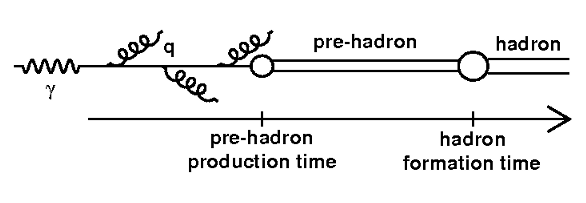
\includegraphics[width=10cm] {fig/hadro.png} 
\caption {Sketch of the hadronization process.}
\label{fig:hadro}
\end{figure}

The hadronization in nuclear matter is a key process of the Quantum Chromo-Dynamics theory (QCD) because it leads to major theoretical uncertainties in numerous measurements. As the nuclear medium is hot and evolving in Relativistic Heavy Ion Collisions (RHIC), DIS experiments at JLab energies are well suited to test different theoretical models, including the RHIC's ones, because the size of cold nuclei is stable and known. A quantitative understanding of the hadronization process in nuclei is also an interesting theme for neutrino experiments that often use nuclei to maximize their cross sections. The hadronization can give an important information about nuclei through the quark energy loss, for example, Arleo's model~\cite{Arleo:2003yf} correlates the quark energy loss with a gluon density, and Kopeliovich et al.'s model~\cite{Kopeliovich:2010aa} correlates the $\Delta \langle P_T^2 \rangle$ with the saturation scale. Other models \cite{Gallmeister:2007an} utilize different assumptions to describe the pre-hadron evolution into a full hadron. Therefore, high precision measurements are very important to discriminate between different models. 

In order to constrain the existing models we extracted our results using a tight multi-dimensional binning. That was viable due to the high statistics of our EG2 data, which allowed the study of both pions production over a wide kinematic range.

We present in section \ref{sec:theo} a highlight of different models' families describing the hadronization process in hot and cold nuclear matter, then in section \ref{sec:exp} we make a rapid overview of published results. For more detailed information, we refer the readers to the review of Accardi {\it et al.} \cite{Accardi:2009qv}.


\subsection{Kinematic Variables and Observables}

In this analysis we use the following Semi-Inclusive Deep Inelastic Scattering (SIDIS) variables:
\begin{itemize}
 \item $\nu = E_i - E_f$ is the energy transferred by the lepton probe in the laboratory frame, where $E_i$ is the beam energy and $E_f$ is the scattered electron energy,
 \item $Q^2 = 4 E_i E_f \sin ^2(\theta_e / 2)$ is the 4-momentum transferred, with $\theta_e$ is the polar angle of a scattered electron,
 \item $x_{Bj} = {{Q^2} \over {2 M_n \nu}}$ is the proton momentum fraction carried by the struck quark, with $M_n$ is the nucleon mass,
 \item $W^2 = M_n^2 - Q^2 + 2 M_n \nu$ is the mass squared of the hadronic final state,
 \item $z_h = E_h / \nu$ is the virtual photon energy fraction carried by the measured hadron, with $E_h$ is the hadron energy,
 \item $P_T^2$ is the hadron transverse momentum measured with regard to the virtual photon direction,
 \item $\phi_h$ is the angle between the leptonic plane (containing initial and scattered electrons) and the hadronic plane (containing the virtual photon and a measured hadron),
 \item $x_F = P_L/P_L^{max}$ is the longitudinal momentum fraction carried by the hadron, and calculated with respect to the virtual photon direction in the laboratory frame.
\end{itemize}
%TODO Add t

We define the multiplicity ratio as:
\begin{equation}
R_A^h (Q^2,\nu,z_h,P_T^2) = {{N_A^h (Q^2,\nu,z_h,P_T^2) / N_A^e (Q^2,\nu)} 
                       \over {N_D^h (Q^2,\nu,z_h,P_T^2) / N_D^e (Q^2,\nu)}},
\end{equation}
$N^e_A$ and $N_A^h$ are the number of electrons and semi-inclusive hadrons $h$ measured simultaneously on a target $A$. The multiplicity ratio represents the attenuation of the hadron $h$ in a nuclear target~$A$.
\newline

We define the transverse momentum broadening as:
\begin{equation}
\Delta \langle P_T^2 \rangle = \langle P_T^2 \rangle_A - \langle P_T^2 \rangle_D,
\end{equation}
where $\langle P_T^2 \rangle_A$ is the mean transverse momentum measured on a target $A$.


\subsection{Theoretical Efforts}
\label{sec:theo}

The different models explaining the data can be separated in three families;
some assume that the quark looses energy in the medium and that either the hadronization occurs outside the medium or the hadronic interaction is 
negligible, others neglect the quark energy loss and consider
only the hadron and pre-hadron absorption, and the third category considers both
interactions. For illustration, we will give an example of each case, but for more detailed information, we refer the readers again to our reference~\cite{Accardi:2009qv}, which is more exhaustive and highlights also models describing RHIC's experiments.

In \cite{Wang:2002ri}, E.~Wang and X.-N.~Wang, described HERMES data using only 
the parton energy loss, hence the observed suppression is due to the fact that a lower energy quark fragments into a low number of hadrons at a very low $z$. This kind of models is suitable for both RHIC and nDIS experiments since it permits a common interpretation of hadron suppression in the nuclear matter. Moreover, various calculations have described the parton energy loss in the nuclear medium using the $\hat q$ (GeV$^2$ fm$^{-1}$) parameter, that is defined as the quark transverse momentum normalized by its propagation path length. In these models, $\hat q$ is mainly related to the $P_T$ broadening observable. The main difficulty of quark energy loss models is the lack of a coherent description for both multiplicity ratios and $P_T$ broadening behaviors. Recent models used a $\hat q$ to reproduce multiplicity ratio, which is too large to describe the transverse momentum broadening.
% TODO Add a ref

The other transport model, GiBUU~\cite{Gallmeister:2007an}, is based on the 
Boltzmann equation that employs hadronic and pre-hadronic interactions in the nuclear matter without involving any quark energy loss. This model reproduces very well most of hadrons' multiplicity ratios, however, it failed to describe the transverse momentum broadening. 
%$\Delta \langle P_T^2 \rangle$ variable is not described at all by 

Furthermore, B.Z.~Kopeliovich et al. \cite{Kopeliovich:2008uy} described the process by neither neglecting the quark energy loss nor the hadron absorption, but used both $\Delta \langle P_T^2 \rangle$ and $R_A^h$ observables to differentiate between these effects. In that case, the transverse momentum broadening is correlated with the quark energy loss, and the suppression of multiplicity ratios is explained by the hadron absorption in the nuclear medium.

To conclude it is important to point out that no consensus is reached on which 
mechanisms are dominant. It is, therefore, important to perform precise measurements with the appropriate observables to disentangle these effects.


\subsection{Previous Mesurements}
\label{sec:exp}

Hadron multiplicity ratios in nuclei were measured in numerous lepton 
facilities: L.S.~Osborne {\it et al.} \cite{Osborne:1978ai} at SLAC,
L.~Hand {\it et al.} \cite{Hand:1978tx}, the E665 collaboration \cite{Adams:1994ri} at FNAL, and the European Muon Collaboration \cite{Arvidson:1984fz,Ashman:1991cx} at CERN. These measurements revealed the main features of the hadronization mechanism
in nuclei by showing a suppression of hadrons' production in heavy nuclei.
This suppression appears to be reduced at higher $\nu$ and lower $z$, and it 
can even inverse sign and become an increased yield at very low $z$. 

Figures \ref{fig:her1}, \ref{fig:her2} and \ref{fig:her3} show a sample of 
the most recent HERMES data~\cite{Airapetian:2007vu}, where numerous hadrons were individually studied, and new variables linked with the transverse momentum were used in addition to the usual multiplicity ratio.

\begin{figure}[htbp]
\centering
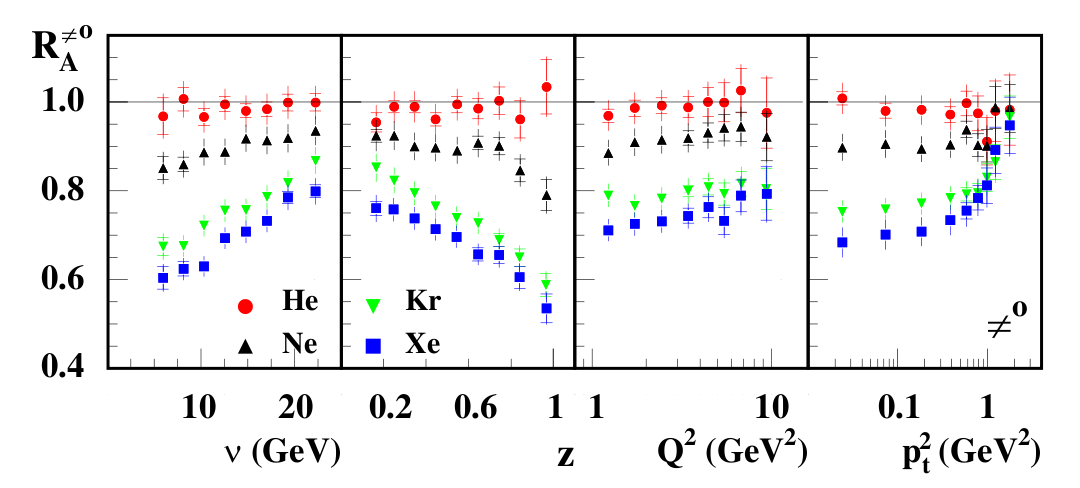
\includegraphics[width=14cm] {fig/Hermes/pi0hermes.png} 
\caption {Multiplicity ratios of $\pi^0$ as a function of various kinematical variables from the HERMES collaboration \cite{Airapetian:2003mi}}
\label{fig:her1}
\end{figure}

\begin{figure}[htbp]
\centering
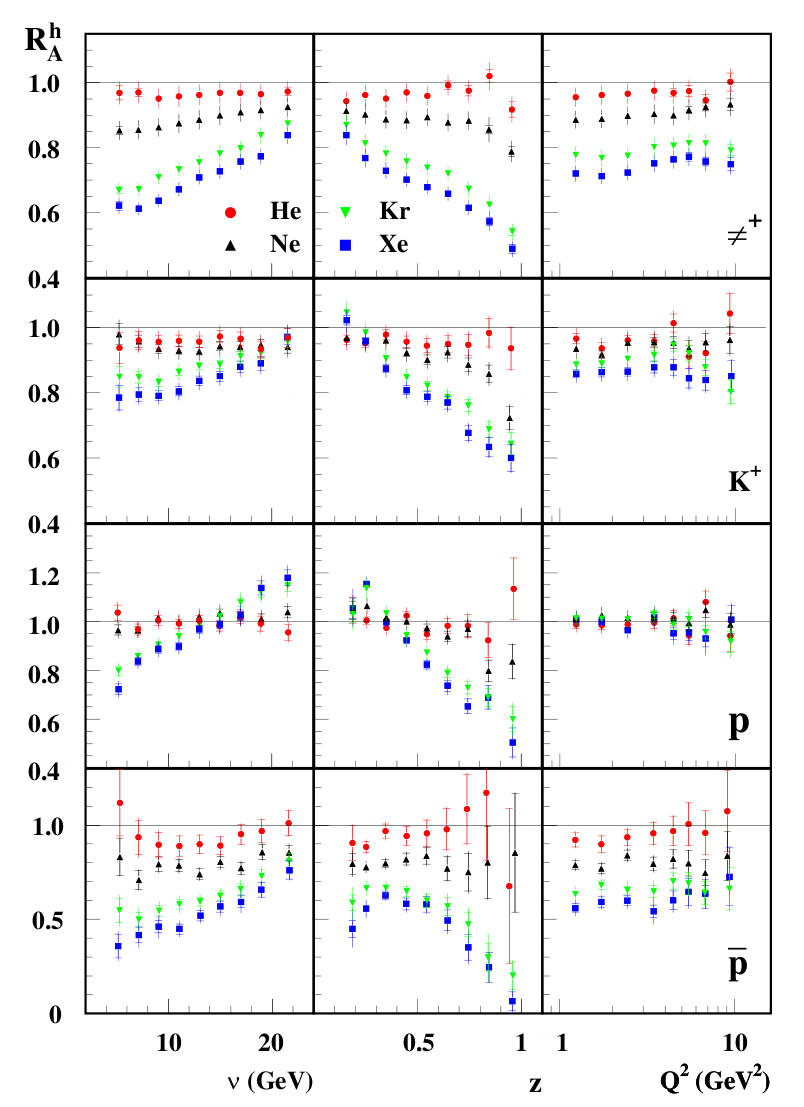
\includegraphics[width=14cm] {fig/Hermes/hermes1.png} 
\caption {Multiplicity ratios of $\pi^+$, K$^+$, protons and anti-protons as a 
function of various kinematical variables from the HERMES collaboration \cite{Airapetian:2007vu}}
\label{fig:her2}
\end{figure}

\begin{figure}[htbp]
\centering
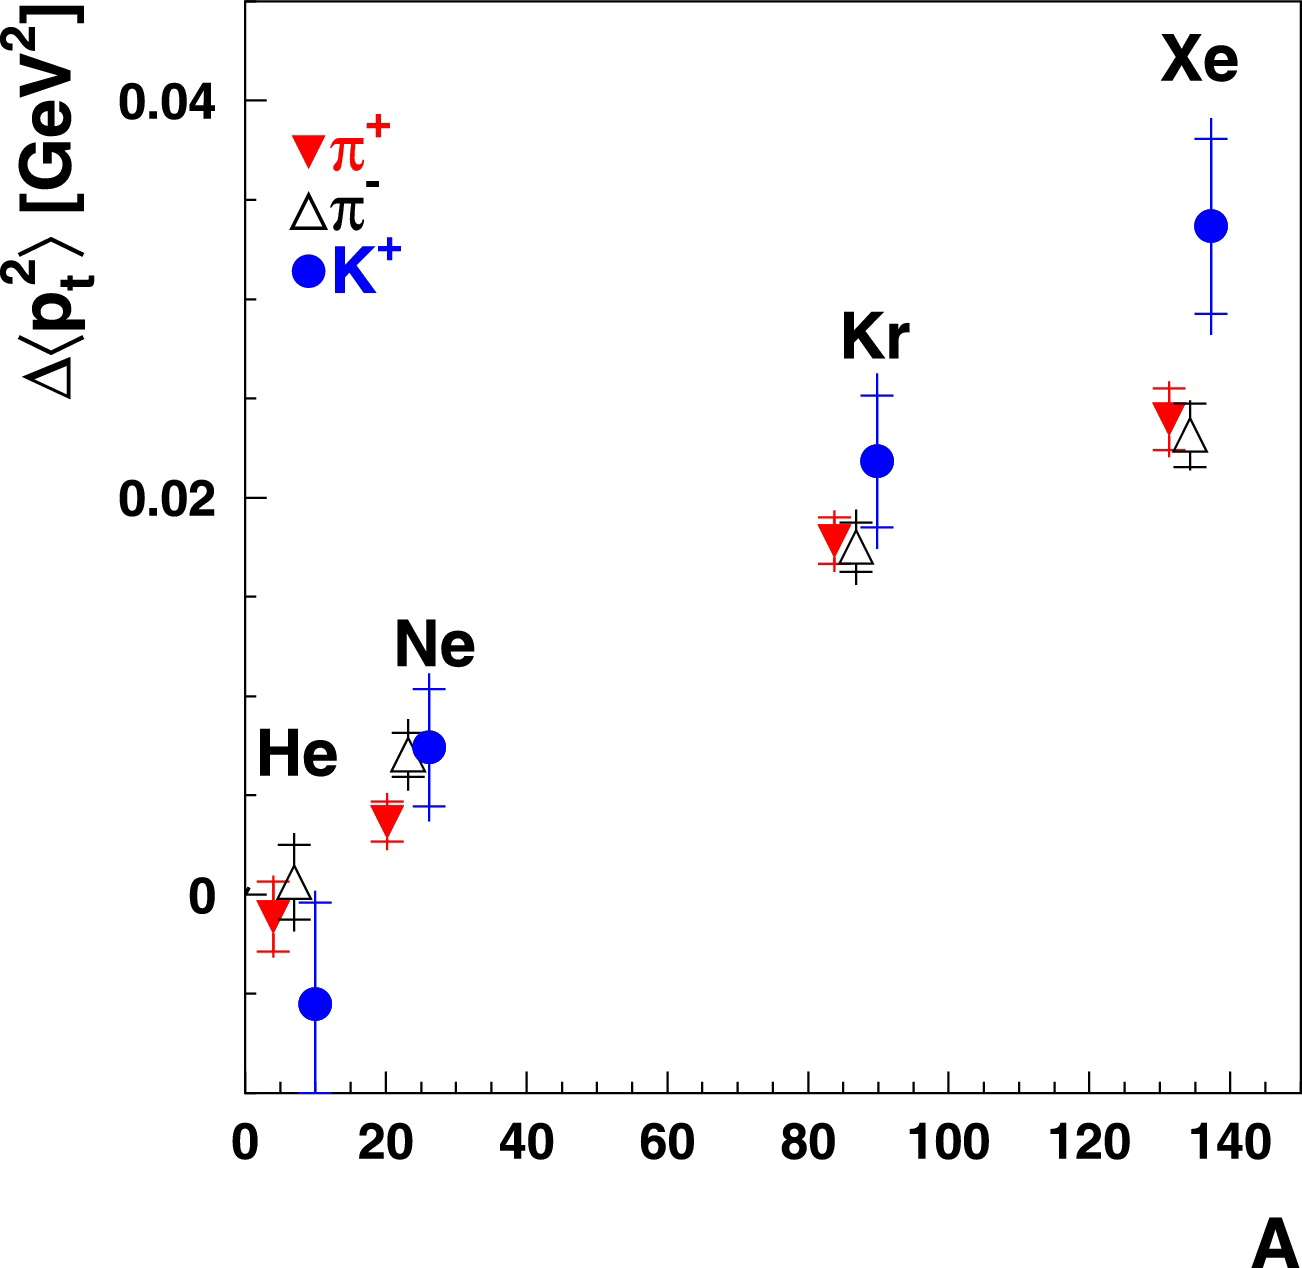
\includegraphics[width=7cm] {fig/Hermes/pthermes.png} 
\caption {Transverse momentum broadening for various particles from the HERMES collaboration \cite{Airapetian:2009jy}}
\label{fig:her3}
\end{figure}

The good precision of HERMES data shed light on new hadronization features, such as the behavior of K$^+$s, which have less attenuation than pions (see figure \ref{fig:her1}) but an excess on $\Delta \langle P_T^2 \rangle$. Must note that it is difficult to reproduce this behavior on models where only one hadronization stage is taken into account to explain all effects. Likewise, the different behavior of protons compared to anti-protons (see figure \ref{fig:her2}) is interesting and needs more precise analyses to unravel it since most of the existing models do not treat yet the baryons' hadronization.

